% Data flow diagram
% Author: David Fokkema
\documentclass{article}
\usepackage{tikz}
\usetikzlibrary{shapes,arrows}
\usepackage{pdflscape}
\usepackage[papersize={12cm, 10.1cm}, text={15cm, 10.2cm}]{geometry}
\usetikzlibrary{decorations.text}
\usepackage{xcolor}
% \selectcolormodel{gray}

\begin{document}
\thispagestyle{empty}
%\begin{landscape}
\begin{center}
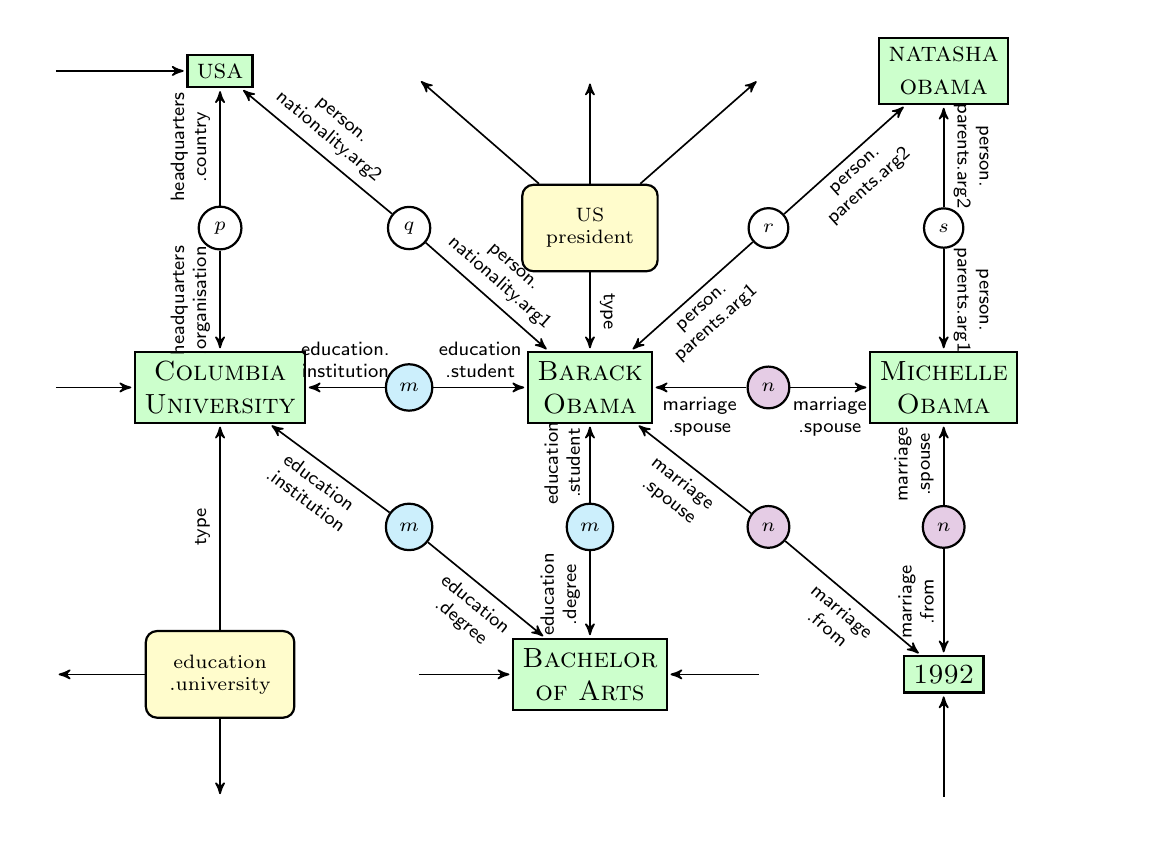
\begin{tikzpicture}[
  font=\sffamily,
  every matrix/.style={ampersand replacement=\&,column sep=1cm,row sep=1cm,font=\scriptsize},
  entity/.style={draw,thick,rectangle,fill=green!20,font=\sc},
  word/.style={draw,thick,ellipse,fill=blue!20,font=\sc},
  emptyNode/.style={},
  mediator/.style={draw,thick,circle},
  mediatorC/.style={draw,thick,circle,fill=cyan!20},
  mediatorV/.style={draw,thick,circle,fill=violet!20},
  mediatorY/.style={draw,thick,circle,fill=yellow!20},
  entityType/.style={draw,thick,rounded corners,fill=yellow!20,inner sep=.3cm},
  mathType/.style={draw,thick,diamond,fill=red!20},
  mediatorToEntity/.style={->,>=stealth',shorten >=1pt,semithick,black,sloped,above,font=\sffamily\scriptsize},
  typeToEntity/.style={->,>=stealth',shorten >=1pt,semithick,black,sloped,above,font=\sffamily\scriptsize},
  wordToEntity/.style={-,>=stealth',shorten >=1pt,ultra thick,dotted,blue,sloped,above,font=\sffamily\scriptsize},
  entityToMath/.style={->,>=stealth',shorten >=1pt,ultra thick,dashed,violet,sloped,above,font=\sffamily\scriptsize},
  every node/.style={align=center}]

  
  % Edinburgh is the capital of Scotland 
  
  % Position the nodes using a matrix layout
  \matrix{
%   \node[emptyNode] (e1) {}; \& \node[entity] (usa) {usa}; \& \node[emptyNode] (e2) {}; \& \node[emptyNode] (e3) {}; \& \node[emptyNode] (e4) {}; \& \node[entity] (natasha) {natasha\\obama}; \& \node[emptyNode] (e5) {};\\
%                             \& \node[mediator] (m1) {1}; \& \node[mediator] (m2) {2}; \& \node[entityType] (president) {US\\president}; \& \node[mediator] (m3) {3}; \& \node[mediator] (m4) {4}; \& \\
%   \node[emptyNode] (e6) {}; \& \node[entity] (columbia) {Columbia\\University}; \& \node[mediatorC] (m5) {5}; \& \node[entity] (obama) {Barack\\Obama}; \& \node[mediatorV] (m6) {6}; \& \node[entity] (michelle) {Michelle\\Obama};  \& \node[emptyNode] (e7) {};\\ 
%   \& \& \node[mediatorC] (m7) {7}; \& \node[mediatorC] (m8) {8}; \& \node[mediatorV] (m9) {9}; \& \node[mediatorV] (m10) {10}; \& \\
%   \node[emptyNode] (e8) {}; \& \node[entityType] (university) {education\\.university}; \& \node[emptyNode] (e9) {}; \& \node[entity] (ba) {Bachelor\\of Arts}; \& \node[emptyNode] (e10) {}; \& \node[entity] (1992) {1992}; \& \node[entityType] (female) {gender\\.female}; \\ 
%   \& \node[emptyNode] (e11) {}; \&  \&  \&  \& \node[emptyNode] (e12) {}; \&  \node[emptyNode] (e13) {}; \\
  
  \node[emptyNode] (e1) {}; \& \node[entity] (usa) {usa}; \& \node[emptyNode] (e2) {}; \& \node[emptyNode] (e3) {}; \& \node[emptyNode] (e4) {}; \& \node[entity] (natasha) {natasha\\obama};  \\
                            \& \node[mediator] (m1) {$p$}; \& \node[mediator] (m2) {$q$}; \&
\node[entityType] (president) {US\\president}; \& \node[mediator] (m3) {$r$}; \& \node[mediator]
(m4) {$s$};  \\
  \node[emptyNode] (e6) {}; \& \node[entity] (columbia) {Columbia\\University}; \& \node[mediatorC]
(m5) {$m$}; \& \node[entity] (obama) {Barack\\Obama}; \& \node[mediatorV] (m6) {$n$}; \&
\node[entity] (michelle) {Michelle\\Obama};   \\ 
  \& \& \node[mediatorC] (m7) {$m$}; \& \node[mediatorC] (m8) {$m$}; \& \node[mediatorV] (m9) {$n$};
\& \node[mediatorV] (m10) {$n$}; \\
  \node[emptyNode] (e8) {}; \& \node[entityType] (university) {education\\.university}; \& \node[emptyNode] (e9) {}; \& \node[entity] (ba) {Bachelor\\of Arts}; \& \node[emptyNode] (e10) {}; \& \node[entity] (1992) {1992}; \\ 
  \& \node[emptyNode] (e11) {}; \&  \&  \&  \& \node[emptyNode] (e12) {}; \&  \node[emptyNode] (e13) {}; \\
  };
 
 
 
 \draw [mediatorToEntity] (m1) edge node {headquarters\\.country}  (usa);
 \draw [mediatorToEntity] (m1) edge node[rotate=180] {headquarters\\.organisation}  (columbia);
 
 \draw [mediatorToEntity] (m2) edge node {person.\\nationality.arg2}  (usa);
 \draw [mediatorToEntity] (m2) edge node {person.\\nationality.arg1}  (obama);
 
 \draw [mediatorToEntity] (m3) edge node[below] {person.\\parents.arg2}  (natasha);
 \draw [mediatorToEntity] (m3) edge node[below] {person.\\parents.arg1}  (obama);
 
 \draw [mediatorToEntity] (m4) edge node[rotate=180] {person.\\parents.arg2}  (natasha);
 \draw [mediatorToEntity] (m4) edge node {person.\\parents.arg1}  (michelle);
 
 \draw [mediatorToEntity] (m5) edge node {education.\\institution}  (columbia);
 \draw [mediatorToEntity] (m5) edge node {education\\.student}  (obama);
 
 \draw [mediatorToEntity] (m6) edge node[below] {marriage\\.spouse}  (michelle);
 \draw [mediatorToEntity] (m6) edge node[below] {marriage\\.spouse}  (obama);
 
 \draw [mediatorToEntity] (m7) edge node[below] {education\\.institution}  (columbia);
 \draw [mediatorToEntity] (m7) edge node[below] {education\\.degree}  (ba);
 
 \draw [mediatorToEntity] (m8) edge node[rotate=180] {education\\.degree}  (ba);
 \draw [mediatorToEntity] (m8) edge node {education\\.student}  (obama);
 
 \draw [mediatorToEntity] (m9) edge node[below] {marriage\\.from}  (1992);
 \draw [mediatorToEntity] (m9) edge node[below] {marriage\\.spouse}  (obama);
 
 \draw [mediatorToEntity] (m10) edge node[rotate=180] {marriage\\.from}  (1992);
 \draw [mediatorToEntity] (m10) edge node {marriage\\.spouse}  (michelle);
 
 
 % empty nodes
 \draw [mediatorToEntity] (e1) edge node {}  (usa);
 \draw [mediatorToEntity] (president) edge node {}  (e2);
 \draw [mediatorToEntity] (president) edge node {}  (e3);
 \draw [mediatorToEntity] (president) edge node {}  (e4);
 % \draw [mediatorToEntity] (e5) edge node {}  (natasha);
 \draw [mediatorToEntity] (e6) edge node {}  (columbia);
 % \draw [mediatorToEntity] (e7) edge node {}  (michelle);
 \draw [mediatorToEntity] (university) edge node {}  (e8);
 \draw [mediatorToEntity] (e9) edge node {}  (ba);
 \draw [mediatorToEntity] (e10) edge node {}  (ba);
 \draw [mediatorToEntity] (university) edge node {}  (e11);
 \draw [mediatorToEntity] (e12) edge node {}  (1992);
 % \draw [mediatorToEntity] (female) edge node {}  (e13);
   
  % type to entity
  \draw [typeToEntity] (university) edge node {type}  (columbia);
  \draw [typeToEntity] (president) edge node {type}  (obama);
  % \draw [typeToEntity] (female) edge node {type}  (michelle);
  
\end{tikzpicture} 
\end{center}

% \end{landscape}

% \begin{tikzpicture}
% \node (One) at (-3,0) [shape=circle,draw] {$One$}; 
% \node (Two) at (3,0) [shape=circle,draw] {$Two$};
% \def\myshift#1{\raisebox{-2.5ex}}
% \draw [->,thick,postaction={decorate,decoration={text along path,text align=center,text={|\sffamily\myshift|Some more bent text}}}] (One) to [bend right=45]  (Two);
% \def\myshift#1{\raisebox{1ex}}
% \draw [->,thick,postaction={decorate,decoration={text along path,text align=center,text={|\sffamily\myshift|Some bent text}}}]      (One) to [bend left=45] (Two);
% \end{tikzpicture}


\end{document}
